% !TEX ROOT = ../ersti.tex
\section{Physik 100\%}

\begin{figure}[b]
	\centering
	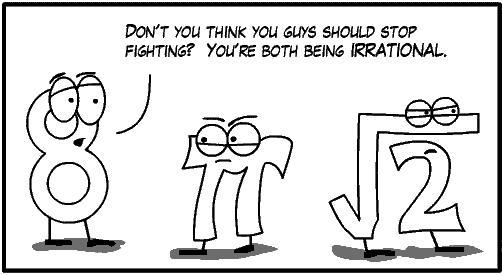
\includegraphics[width=\linewidth]{bilder/both_irrational.png}
\end{figure}

\subsection{Erstes Semester}

Das erste Semester ist, verglichen mit späteren Semestern, sehr stark durchstrukturiert, was euch den Wechsel von der Schule an die Uni erleichtert, jedoch auch nicht besonders viele Freiheiten lässt.  Allgemein werdet ihr bis ins vierte Semester im Pflichtprogramm je eine „Experimentalphysik“ (\gls{Ex}) und eine „Theoretische Physik“ (\gls{Theo})\footnote{Die Abkürzung „Theo“ kann zu Verwirrungen mit Informatikern führen, da diese das als „Theoretische Informatik“ verstehen.} Vorlesung besuchen, wobei im fünften Semester noch die Ex 5 folgt. Zusätzlich dazu hört ihr an Mathe im ersten Semester die „Lineare Algebra 1“ (\gls{LA}) und wenn ihr wollt auch die „Analysis 1“ (\gls{Ana}); aber zur Mathe später mehr.

Das ganze Semester über werdet ihr jede Woche in jeder Vorlesung, die ihr hört, einen Übungszettel bekommen, den ihr dann auf die nächste Woche lösen sollt. Diese dienen zum Einüben des in den Vorlesungen behandelten Stoffes und zugleich häufig als Klausurzulassung. Man benötigt meistens insgesamt 50 - 60 \% der Gesamtpunktzahl auf allen Zetteln, aber wenn es nur um ein paar Punkte geht, sind die Tutorinnen meistens kulant. Wenn eure Tutorin den Eindruck hat, ihr verschwendet mit der Klausur keinen Prüfungsversuch, lässt sie euch meistens zu. Macht euch darum aber erstmal keinen Kopf, wenn ihr am Ball bleibt, ist das überhaupt kein Problem, ihr müsst sie ja nicht alle alleine lösen.

\subsection{Orientierungsprüfung}

Die Orientierungsprüfung ist eine Prüfung, die ihr bis zum Ende des 3. Semesters bestehen müsst, um weiterhin Physik studieren zu dürfen. Im Bachelor Physik ist dies die ganz normale Klausur in der Ex 1. Dort werden meist sehr schulnahe physikalische Grundlagen der Mechanik behandelt. Macht euch also keine Sorgen. Das schafft ihr!

\subsection{Basiskurs}

Der Basiskurs beginnt, wie ihr wahrscheinlich schon wisst, in der letzten Vorkurswoche und soll euch den Einstieg in das Studium erleichtern. Dabei werden euch sogenannte Schlüsselkompetenzen beigebracht, die euch unter anderem in Zeitmanagement, Literatursuche und das Textsatzsytem \LaTeX{} einführen. Auch wenn ihr vermutlich schon einiges davon kennt, ist es doch ganz nett, nochmal alles kompakt zu sehen und vor allem dabei neue Menschen und vielleicht auch spätere „Zettelpartnerinnen“ kennenlernen zu können. Leider ist die Qualität des Kurses oft stark abhängig von eurer Tutorin. Ihr müsst also für euch bestimmen, wie viel ihr aus diesem Kurs mitnehmt. Bedenkt, die Tutorin bekommt Geld für diesen Kurs, ihr dürft also auch etwas von ihr erwarten und ihr ganz viele Fragen stellen.

\subsection{Analysis vs. Höhere Mathematik für \\Physiker}
Ihr habt zwei Möglichkeiten, die für das Studium benötigte Analysis zu erlernen.
In der ersten Variante hört ihr im zweiten Semester die Vorlesung „Höhere Mathematik für Physiker 2“\footnote{Es gibt keine „Höhere Mathematik für Physiker 1“, weil die Vorlesungen parallel zur Ana 2 und Ana 3 laufen. Die Lineare Algebra im ersten Semester gilt sozusagen als die HöMa 1.} (\gls{HoMa}) und im dritten Semester „Höhere Mathematik für Physiker 3“. Alternativ dazu könnt ihr im zweiten Semester Ana 2 und im dritten Semester Ana 3 hören. Falls ihr euch dafür entscheidet, empfiehlt es sich stark, zusätzlich im ersten Semester die Vorlesung Ana 1 zu hören, da diese die fachliche Grundlage für Ana 2 und Ana 3 bietet. Diese Problematik wird im \autoref{mathephysik} weiter diskutiert.

\subsection{Weiteres Studium}

Euer weiteres Studium sieht, wie oben kurz angedeutet, so aus, dass ihr immer ein Grundgerüst an Vorlesungen habt und euch darum herum andere Vorlesungen und Seminare selbst auswählen könnt. Die Experimentalphysikvorlesungen sind bis zum fünften Semester und die theoretischen bis zum vierten Semester Pflicht. Hinzu kommen im zweiten und dritten Semester entweder die HöMa 2 und 3, oder die Ana 2 und 3. Ansonsten seid ihr jedoch bis auf ein Pflichtseminar, das ihr aus einem relativ großen Topf an Seminaren auswählen könnt und den Pflichtpraktika frei alles zu hören, was euch so in den Sinn kommt. Ihr müsst einzig darauf achten, dass ihr in den einzelnen Bereichen ausreichend „Punkte sammelt“: Im Wahlpflichtbereich sind das 14 \gls{LP}, bei den Übergreifenden Kompetenzen 19 \gls{LP} und im Wahlbereich bis zu 17 \gls{LP}. Nutzt frühzeitig die Gelegenheit Veranstaltungen zu besuchen, die euch interessieren, dann macht das Studium gleich doppelt so viel Spaß!

\begin{figure}[b]
	\centering
	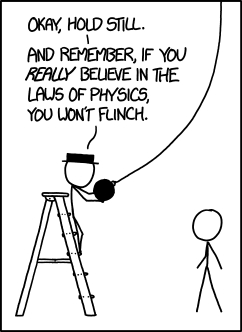
\includegraphics[width=.75\linewidth]{bilder/laws_of_physics.png}
\end{figure}

\subsection{Wahlbereich, Wahlpflichtbereich und \\Übergreifende Kompetenzen}

Im Laufe eures Bachelorstudiums müsst ihr ggf. ein oder zwei Wahlfächer belegen, welche ihr aus einem recht weit gefächerten Angebot wählen könnt. Diese Wahlfächer müssen auch nicht zwingendermaßen aus Bereichen der Physik kommen, sondern können z.B. Mathe, Chemie oder Philosophie sein. Was ihr alles für Möglichkeiten habt, könnt ihr genauer in der Prüfungsordnung nachlesen und selbst Fächer, die dort nicht aufgezählt sind, lassen sich möglicherweise nach Absprache mit dem Prüfungsausschuss auch anrechnen lassen.\\

Der Wahlpflichtbereich besteht, im Gegensatz zum Wahlbereich und den Übergreifenden Kompetenzen, aus vertiefenden oder weiterführenden Physikveranstaltungen. Schaut doch einfach in das Vorlesungsverzeichnis im LSF und sucht euch interessante Vorlesungen oder auch Seminare aus. Besonders Seminare können viel Spaß machen, da diese zwar oftmals viel selbstständiges Arbeiten verlangen, aber oft auch forschungsnäher sind als Vorlesungen. Zudem findet ihr auch Anregungen dazu in der Prüfungsordnung und im Modulhandbuch.\\

Der Bereich Übergreifende Kompetenzen soll euch ein wenig dazu bewegen fachunabhängige Kompetenzen zu erlernen. Darunter fallen der mathematische Vorkurs, der Basiskurs, sowie alle als „Überfachliche Kompetenzen“ gekennzeichneten Module der Mathematik, Informatik und den Naturwissenschaften. Außerdem lassen sich oft nach Rücksprache mit dem Prüfungssekretariat auch weitere Veranstaltungen anrechnen lassen, wie zum Beispiel Sprachkurse, Programmierkurse, usw.\\

Allgemein gilt: Versucht, möglichst früh Dinge aus Gebieten, die euch wirklich interessieren, zu hören; denn das sind die Fächer die euch auch wirklich Spaß machen und ihr erlangt ein möglichst breites, und vor allem tiefes Wissen, welches euch bei eurer Bachelorarbeit und vermutlich auch sonst zugutekommt.

\subsection{Prüfungen und Noten}

Es wird euch sicher freuen zu hören, dass eine nicht bestandene Klausur nicht gleich das Ende für euer Studium bedeutet. Im Grunde ist die Wiederholungsregelung sogar recht studifreundlich; so habt ihr in jedem Modul zwei Versuche, wobei in der Regel ein Versuch aus einer Klausur und, wenn nötig, der dazugehörenden Nachklausur besteht. Darüber hinaus habt ihr für euer Studium noch zwei sogenannte Joker, die euch jeweils einen dritten Versuch geben, falls die zwei regulären nicht reichen sollen (dies gilt nicht für eure Orientierungsprüfung, welche die Prüfung in der Ex 1 darstellt). Darüber hinaus ist für euch recht interessant, dass es die Möglichkeit gibt, zwei Noten aus unterschiedlichen Bereichen der tendenziell schlechteren Pflichtmodule zu streichen. Macht euch also nicht zu viele Gedanken darüber, wenn eure Noten zunächst nicht ganz so gut sind. Auch könnt ihr jederzeit zusätzlich gehörte Module in den Zusatzqualifikationenbereich verschieben, wenn ihr diese nicht benötigt, euch entsteht also kein Nachteil dadurch, dass ihr mehr hört, als ihr müsst.\\

Sonst ist noch zu erwähnen, dass ihr, um in Heidelberg in den Master zugelassen zu werden, eine Bachelornote von 2,9 oder besser braucht. Das war bisher bislang noch nie ein Problem für Heidelberger Studis, der Notenschnitt liegt durchschnittlich zwischen 1,7 und 2,0.

\subsection{Regel- und Maximalstudienzeit}

Vielleicht ist euch das ominöse Wort „Regelstudienzeit“ vor eurem Studium bereits zu Ohren gekommen. An dieser Stelle wollen wir mit ein paar Mythen, die sich um sie ranken, aufräumen.\\
Obwohl das Wort an sich es suggeriert, ist es keinesfalls die Regel, dass Studierende ihr Studium in Regelstudienzeit abschließen. Es handelt sich also nicht um die durchschnittliche Studiendauer, welche je nach Fach mehr oder weniger deutlich über den vorgesehenen sechs Semestern für den Bachelor und vier für den Master liegen. Die Regelstudienzeit gibt lediglich an, wie schnell man ein Studium abschließen kann, wenn man jedes Semester im Schnitt 30 Leistungspunkte absolviert. Die Fakultäten gehen dabei die Selbstverpflichtung ein, dass ein Studium in der Regelstudienzeit studierbar ist.
Die Gründe für ein längeres Studium sind vielfältig, neben Lohnarbeit zur Finanzierung des Studiums oder nicht bestandenen Prüfungen sind diese auch nicht alle negativ konotiert. So hören viele Studierende aus Interesse zusätzliche Vorlesungen bevor sie ihre Abschlussarbeit abschließen. Intensives ehrenamtliches Engagement, z.B. in der Hochschulpolitik kann ebenfalls ein Grund sein. Ebenfalls ist es üblich, dass ein Auslandsaufenhalt im Studium zu einer Verlängerung des Studiums führt. 
Wie ihr seht ist es also ein weit verbreiteter Irrglaube, dass nur faule oder schlechte Studentinnen länger als vorgesehen studieren würden. Die Universität ist nun Mal kein Ausbildungsbetrieb im klassischen Sinne, sondern dient neben dem Erwerb fachlicher Kompetenzen auch dem Entwickeln der Persönlichkeit und dem interdisziplinären Wissenserwerb. Die Universität ist eine unvergleichliche Lernumgebung, auf die man, einmal im Arbeitsleben angelangt, mit Sehnsucht zurückschaut. Die Mentalität die wir euch ans Herz legen wollen ist, dass ihr euch nicht unter Druck setzen lasst und das Studium in der euch angemessen erscheinenden Zeit absolviert.
Es gibt dabei jedoch zwei Wermutstropfen. Der Bafög-Anspruch ist auf das Studium in Regelstudienzeit beschränkt, es gibt jedoch viele Möglichkeiten, bis zu zwei Semester pro Studienabschnitt länger Bafög zu beziehen. Ebenfalls sei angemerkt, dass die Physik in ihrer Prüfungsordnung verankert hat, dass man dass man die letzte Prüfungsleistungen spätestens im dritten Semester nach Überschreiten der Regelstudienzeit absolvieren muss, was eine Maximalstudiendauer von neun Semestern im Bachelor entspricht. Wenn man diese überschreitet müsste man also formal gesehen exmatrikuliert werden, in der Realität wird dies jedoch nach unserem Stand nie durchgezogen. Die Fakultät hat kein Interesse daran, Personen die in ihrem zehntem Semester kurz vor dem Abschluss stehen zu exmatrikulieren. Diese Grenze wird viel mehr als eine notwendige extrinsische Motivation angesehen, zielstrebig zu studieren. Macht euch deswegen also keinen Kopf!

\subsection{Prüfungsordnung und Modulhandbuch}

\begin{figure*}[b]
    \centering{
    \includegraphics[width=\textwidth]{bilder/purity.png}
}
\end{figure*}

Immer dann, wenn sich euch Fragen zu eurem Studium stellen oder ihr euch einfach über den weiteren Studienverlauf informieren wollt, sind die ersten Anlaufstellen die Prüfungsordnung und das Modulhandbuch. In der Prüfungsordnung ist formal geregelt, wie der Studienablauf, die Prüfungen und die Anrechenbarkeit von Modulen aussehen. Das Modulhandbuch wiederum ist im Großen und Ganzen eine Auflistung der in der Physik (und benachbarten Gebieten) angebotenen Veranstaltungen. Zurzeit findet ihr beide Dokumente auf der Hauptseite des Bachelors Physik. Leider ist das Modulhandbuch oft nicht ganz aktuell, falls euch Verbesserungen auffallen, meldet euch einfach bei uns.\\

Ansonsten könnt ihr auch gerne zu uns in die Fachschaft auf eine Tasse Kaffee oder Tee vorbeikommen. In vielen Fällen können wir euch auch weiterhelfen.

